%%%%%%%%%%%%%%%%%%%%%%%%%%%%%%%%%%%%%%%%%%%%%%%%%%%%%%%%%%%%%%%%%%%%%
% LaTeX Template: Project Titlepage Modified (v 0.1) by rcx
%
% Original Source: http://www.howtotex.com
% Date: February 2014
% 
% This is a title page template which be used for articles & reports.
% 
% This is the modified version of the original Latex template from
% aforementioned website.
% 
%%%%%%%%%%%%%%%%%%%%%%%%%%%%%%%%%%%%%%%%%%%%%%%%%%%%%%%%%%%%%%%%%%%%%%

\documentclass[12pt]{article}
\usepackage[a4paper]{geometry}
\usepackage[myheadings]{fullpage}
\usepackage{fancyhdr}

\usepackage{lastpage}
\usepackage{graphicx, wrapfig, subcaption, setspace, booktabs}
\usepackage[utf8]{inputenc}
\usepackage[T1]{fontenc}
%\usepackage[font=small, labelfont=bf]{caption}
\usepackage{fourier}
\usepackage[protrusion=true, expansion=true]{microtype}
\usepackage[french]{babel}
\usepackage{sectsty}
\usepackage{url, lipsum}


\newcommand{\HRule}[1]{\rule{\linewidth}{#1}}
\onehalfspacing
\setcounter{tocdepth}{5}
\setcounter{secnumdepth}{5}

%-------------------------------------------------------------------------------
% HEADER & FOOTER
%-------------------------------------------------------------------------------
\pagestyle{fancy}
\fancyhf{}
\setlength\headheight{15pt}
\fancyhead[L]{Benjamin Sportich Emmanuel de Bézenac}
\fancyhead[R]{UPMC}
\fancyfoot[R]{\thepage\ / \pageref{LastPage}}
%-------------------------------------------------------------------------------
% TITLE PAGE
%-------------------------------------------------------------------------------

\begin{document}

\title{ \normalsize \textsc{MOGPL}
		\\ [2.0cm]
		\HRule{0.5pt} \\
		\LARGE \textbf{\uppercase{LA BALADE DU ROBOT}}
		\HRule{2pt} \\ [0.5cm]
		\normalsize \today \vspace*{5\baselineskip}}

\date{}

\author{
		Benjamin Sportich Emmanuel de Bézenac \\ 
		Université Pierre et Marie Curie \\
		Année Universitaire 2015-2016 }

\maketitle

\newpage
\tableofcontents

\newpage
%-------------------------------------------------------------------------------
% Section title formatting
\sectionfont{\scshape}

\clearpage
\newpage
\section{Introduction}
Nous avons décider de développer le programme en Python pour faciliter la gestion de la mémoire et les listes. Nous avions aussi connaissances des librairies : , facilitant la création, la gestion des graphes ainsi que l'affichage.


\clearpage
\newpage
\section{Formulation du problème}
Intéressons nous d'abord a une seule instance du problème de la balade du robot, c'est-à-dire, étant donné une matrice A de taille $MxN$ oû $\forall i \in {0,...,M-1}$, $\forall j \in {0,...,N-1}$, $A_i,_j=0$, soit $A_i,_j=1$, avec 1 étant défini comme un obstacle, et 0 comme une case libre. Soit O cet ensemble d'obstacles. Nous avons également un point de départ S (et une direction D) et un point d'arrivée E. La question est de trouver un chemin de durée la plus courte, étant donné une matrice A de taille $M.N$ instanciée avec $|O|$ obstacles, d'un point et d'une direction de départ, ainsi qu'un point d'arrivée, sachant que nous pouvons uniquement nous déplacer le long des cases qui sont libres.\\

Pour répondre à cette question, nous avons choisi de formuler le probème sous la forme d'un graphe orienté. Soit $G=(V,E)$ ce graphe orienté, et V et E ses noeuds et ses arcs (respectivement). 

On peut modéliser le problème avec un graphe orienté G=(V,E). 
L'ensemble des nœuds représente l'ensemble des positions possibles du robots sur les rails du grand magasin, c'est à dire sa localisation sur la grille et son orientation. Sauf dans le cas des bords, un quadruplet de nœud n'existe que si le croisement correspondant sur le grillage ne touche aucun obstacle.

Il existe un arc entre le nœud A et le nœud B si et seulement si le robot peut passer de la position correspondant au nœud A à la position correspondant au nœud B en une et une seule commande.

%------------------------------------------------
\clearpage
\newpage
\section{Evalution - Complexité}




Rappelons $G= (V, E)$, notre graphe directionnel associé à un instance du problème. Soit $|O|$ le nombre d'obstacles dans le dépôt. Nous avons donc par construction que $|V| = 4\big((M+1)(N+1)-|O|)$, donc $|V| \le 4(M+1)(N+1)$. De plus, $|E| \le 5|V|$, puisqu'il y a au plus 5 arcs crées à partir d'un noeud: les arcs étiquetés $D, G, a1, a2$, et $a3$. Donc $|E| \le 20(M+1)(N+1).$\\

Complexité de la création du graphe:\\
Un noeud est crée en $O(1)$, et un arc en $O(1)$ donc le graphe est crée en  $O(|E|+|V|)$, ou encore en $O(M.N)$.\\

Complexité du parcours en profondeur:\\
Nous pouvons observer que le parcours en profondeur ne remet jamais un noeud dans la file. Les opérations de mise en file et de sortie de file prennent un temps $O(1)$, ou un temps de $O(|V|)$. Puisqu'on visite visite au plus tout les noeuds dans la liste d'adjacence, le temps total attribué à celui-ci est $O(|E|)$. La complexité du parcours en largeur est donc $O(|E|+|V|)$. Donc pour une instance donnée de taille $M.N$, nous avons donc que le parcours en profondeur du graphe associé est $O(M.N)$.
\\\\
Pour retrouver le plus court chemin à partir de la fin, il faudra parcourir tout les noeuds jusqu'à atteindre le noeud de départ. Cette étape de backtracking est effectuée en $O(|V|)$, donc en $O(M.N)$.\\\\


Complexité de notre méthode :\\
- Etape 0 : Entrée des paramètres/Interface\\
coût : \\
- Etape 1 : Lecture d'un bloc\\
coût : \\
- Etape 2 : Création du graphe correspondant\\
coût :\\
- Etape 3 : Calcul du plus court chemin (Parcours en largeur)\\
coût : \\
- Etape 4 : Traçage du plus court chemin calculé précédemment (BFS)\\
coût : \\
- Etape 5 : Affichage du résultat\\
coût : \\
Ces 6 étapes sont répétées à chaque bloc.\\
La complexité d'un tel algorithme est O( )



\clearpage
\newpage
\section{Essais numériques}

\subsection{En fonction de la taille de la grille}




\subsection{En fonction du nombre d'obstacles}


-------------------------------------------------
\clearpage
\newpage
\section{Interface utilisateur}


\begin{figure}[!ht]
\centering
\centerline{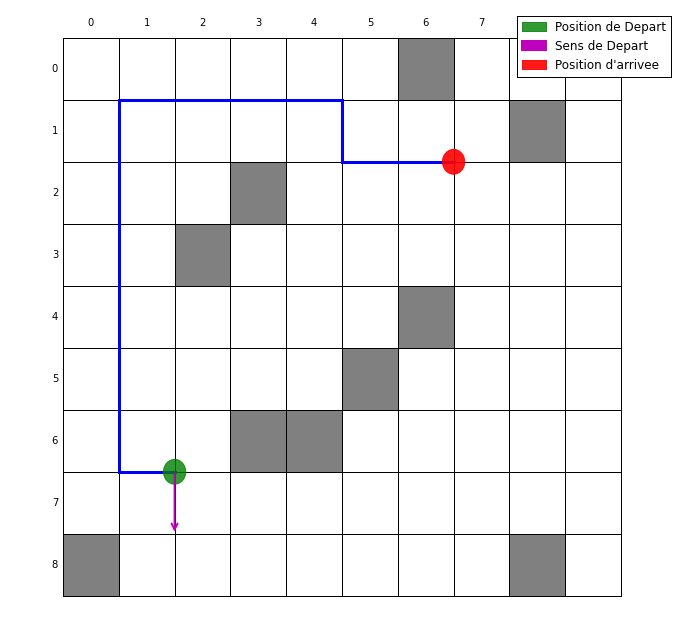
\includegraphics[scale=.4]{example1.png}}
\caption{Interface de la solution du problème énoncé dans le projet.}
\label{ex1}
\end{figure}


\begin{figure}[!ht]
\centering
\centerline{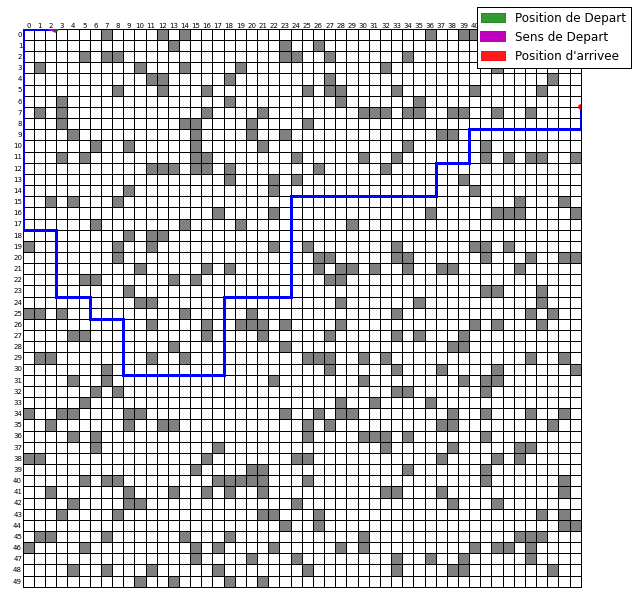
\includegraphics[scale=.6]{example2.png}}
\caption{Exemple d'instance de taille 50, avec  obstacles.}
\label{ex2}
\end{figure}

\clearpage
\newpage
\section{Conclusion}




%Figure : \ref{pouthisteqr}

%\newpage
%\begin{figure}[!t]
%\centering
%\centerline{\includegraphics{moon.jpg}}
%\caption{L'image moon.tif.}
%\label{moontif}
%\end{figure}



\end{document}
